\documentclass[conference]{IEEEtran}

\bibliographystyle{apacite}
% ===========================
% ***              PACKAGES              ***
% ===========================

\usepackage[dvips]{graphicx}
\usepackage{stfloats}
\usepackage{apacite}

\usepackage{color,soul}

\usepackage[cmex10]{amsmath}
\usepackage{amssymb}
\usepackage{mathrsfs}
\usepackage{breqn}
\usepackage{multirow}

\usepackage{tabularx}
\usepackage{multirow}
\usepackage{hhline}

\usepackage{mdwmath}
\usepackage{mdwtab}
\usepackage{pbox}
\usepackage{lipsum}
\usepackage{booktabs,caption,fixltx2e}
\usepackage[flushleft]{threeparttable}
\usepackage{gensymb}


% =============================
% *** HYPHENATION CORRECTION ***
% =============================

\hyphenation{op-tical net-works semi-conduc-tor}


\begin{document}

% =============================
% ***        TITLE AND AUTHORS        ***
% =============================

\title{Terraforming Mars\\The First Steps Towards Making the Planet Inhabitable}

\author{\IEEEauthorblockN{Natasha Ong}
\IEEEauthorblockA{The American School in Japan\\
Tokyo, Japan\\
Email: {18ongn@asij.ac.jp}}}

\maketitle

% =============================
% ***                 ABSTRACT                 ***
% =============================

\begin{abstract}

With the technological advances, humans are getting closer to being able to colonize Mars. However, before the planet can be inhabitable, several terraforming steps must occur. In this paper, we highlight the main challenges, introduce the necessary order of these step with the necessity of creating a magnetic field being the first, and study the properties that need to be fulfilled by the introduction of the magnetic field. We briefly describe some of the existing solutions to creating the magnetic field. Our study shows that though the magnetic field does not need to be very strong, it must be strong enough to protect the planet from solar winds. Several experiments and simulations are run to prove this point. 

\end{abstract}

\IEEEpeerreviewmaketitle


%====================================================%
\section{Introduction}
%====================================================%

Over the past century, human population on Earth has continued to increase, probing scientists to question how much longer Earth will be able to provide the resources to support human life. Thus, scientists and researchers have started to look elsewhere --especially in our solar system-- to possibly colonize, with one of the planets being Mars. From the plants in our solar system, Mars and Venus are the two closest plants to the current habitable zone, shown in Fig. \ref{habitable}. 


However, Venus' surface temperature is about 470 degrees Celcius, extremely hot and unsuitable for human life\cite {}. Moreover, the pressure at the surface is about 90atm, 90 times that of Earth \cite{carroll2017introduction}.  

On the other hand, Mar's proximity to the Sun and its physical aspects, mainly its axial tilt, and rotation rate are most similar to those of Earth, making it a good candidate \cite{mckay1999bringing}. In fact, Earth and Mars have axial tilts of 23.5� and 25� respectively, so Mars?s is within 5 percent of the value for that of Earth\cite{baker2001water}. However, currently, Mars is uninhabitable due to a number of other important factors including its temperature, pressure, and the absence of liquid water on its surface. In fact, the Martian atmosphere could be seen an extremely thin sheet of gas primarily composed of carbon dioxide, with small amounts of nitrogen. On the other hand, Earth's atmosphere is primarily composed of nitrogen and oxygen.

\begin{figure}
   \begin{center}
      \includegraphics[width=9.5 cm]{Figures/habitable_planets.png}
      \caption{Plants in the Solar System in or close to the Habitable Zone}
      \label{habitable}
   \end{center}
\end{figure}

Though it is agreed upon that frozen $CO_2$ exists in the form of dry ice and frozen $H_2O$ exists in the polar caps and soil on the planet, the temperature of the planet's surface must drastically increase for these reserves to be of any use. Specifically, this study will examine the possible ways to terraform Mars by re-establishing its atmosphere, increasing surface temperature, and restoring liquid water. In other words, this study deals with ecopoiesis: planetary engineering to create an anaerobic biosphere to support basic life \cite{fogg1998terraforming}. 

Currently, though some hypothetical processes by which to terraform Mars do exist, they require large amounts of time and effort, as well as budgets. Thus, through \textit{Matlab} and \textit{Universe Sandbox}$^2$, a planetary simulator, the viability of these methods will be examined. 


The remainder of this work is structured as follows: in Section \ref{sec:motiv}, we present our motivations for this work. In Section \ref{sec:requirements}, we list and detail the main requirements needed to make life possible on the planet, and emphasize the importance of the atmosphere. In Section \ref{escape} we discuss the different problems that might lead to the loss of the atmosphere of the planet, which we solve in Section \ref{magnetic}. Section \ref{sec:results} details our experimental results and Section \ref{sec:conclusion} concludes this work.

%====================================================%
\section{Motivations}\label{sec:motiv}
%====================================================%

With scientists and researchers starting to look elsewhere in the universe to possibly colonize, we want to determine which of the methods of terraforming Mars would possibly be viable. A planet's ability to produce an environment capable of supporting life in the long-run would determine whether it can be colonized in the first place. In addition, the pollution, global warming, and rapid population growth make Earth less and less capable of supplying necessary resources.

This research will study the first few steps of terraforming Mars. While there are several factors that influence the possibility of inhabiting Mars long-term, this study will focus on the prerequisites for life --mainly atmosphere, temperature, and water.

%====================================================%
\section{Terraforming Requirements}\label{sec:requirements}
%====================================================%

Terraforming Mars requires different steps. However, some steps have higher priority and must precede others. Specifically, these steps include the establishment of a sufficient atmosphere and surface temperature.

Currently, the atmosphere of Mars is very thin and the atmospheric pressure averages about 0.6\% of that of earth \cite{williams2016}. This atmosphere is composed mainly of Carbon dioxide (i.e., 95.32\%) \cite{williams2016} which, compared to that of Earth, is far from being suitable to sustain human life. However, the composition of Mars's atmosphere is not as critical as its thickness. In fact, since carbon dioxide is an efficient green ouse gas, it might help warm the planet once the terraforming process begins \cite{jakosky2004water}.

%--------------------------------------------------------------%
\subsection{High Surface Pressure}
%--------------------------------------------------------------%

Some studies have shown that the human body cannot survive under very low pressure. The minimum pressure a human body can bear is 0.47 atm \cite{west2002}. While theoretically the minimum threshold altitude for the human body is 8000m, at which the pressure is 0.35 atm \cite{tempest2007}, this pressure is too low and the human body can't stay under such conditions for long. In this study we will assume that the atmosphere of Mars will be thick enough to create an atmospheric pressure equal to 0.57 atm, which is an acceptable pressure under which the human body can live for long enough without risking his life.

%--------------------------------------------------------------%
\subsection{Liquid Water}
%--------------------------------------------------------------%

Nonetheless, to be able to live on Mars, liquid water is required. A long time ago, Mars had an active core, a thicker atmosphere, and a warm climate, allowing for liquid water to exist on its surface. However, when Mars lost its magnetic field and its core started to die, the surface pressure started to decrease, causing the liquid water to either freeze or be evaporated away. Currently, and according to the simplified diagram shown in Fig. \ref{phases}, it is impossible to have liquid water on Mars's surface. A higher pressure is required to get to that point.

\begin{figure}
   \begin{center}
      \includegraphics[width=9.5cm]{Figures/phases.eps}
      \caption{Mars and Earth's conditions in the Pressure Vs Temperature Diagram}
      \label{phases}
   \end{center}
\end{figure}

In literature, different proposals have been suggested to inject various greenhouse gases to start warming the planet \cite{marinova2005}. However, such gases will quickly be blown away by the solar wind, which highlights the importance of maintaining the atmosphere once created.

This requirement highlights the first crucial step: ensuring that the gravity of the planet and its magnetic field are strong enough to maintain the atmosphere.

%--------------------------------------------------------------%
\subsection{Atmosphere Thickness and Gravitation}
%--------------------------------------------------------------%

Mars, has a weak gravitational field given its relatively small size. This makes the molecules in its atmosphere susceptible to being blown away if an external force is applied. In fact, the solar wind and alpha radiation often hit Mars' atmosphere with a strong enough momentum (i.e., they have supersonic speed) to actually remove atmospheric molecules. Furthermore, gravity, weaker at higher altitudes, cannot counter the strong momentum. Thus, only heavy molecules close to the surface remain, due to their weight and distance to the center of mass of Mars. These form the current atmosphere of Mars, a very thin layer of gas.

Earth has a weak gravity as well, which is still strong than Mars's. However, in addition to its gravity, it has a magnetic field that acts like a shield that protects the atmosphere's molecules from the solar wind, and mainly the $\alpha$ particles. This is because these particles have a positive charge $q$ moving on a direction ``almost'' orthogonal to the magnetic field $\vec{B}$ with a velocity $\vec{v}$, which will make them deviate due to the magnetic force $\vec{F}_B = q \vec{v} \bigotimes \vec{B}$, where $\bigotimes$ denotes the cross product.

This highlights the importance of the magnetic field in helping the gravity keep the atmosphere of the planet.

%--------------------------------------------------------------%
\subsection{A Magnetic Field}
%--------------------------------------------------------------%

As explained earlier, a magnetic field is required for Mars to maintain its atmosphere. The magnetic field should be strong enough to deflect the solar wind particles at higher altitudes so that they do not interact with the atmosphere particles. This magnetic field will make the atmosphere's molecules subject only to the gravitation of the planet and the force due to very few particles of the solar wind that go through the magnetic field. However, even those particles will ultimately have a very weak momentum.

%====================================================%
\section{Atmospheric Escape}\label{escape}
%====================================================%

Before discussing the importance of the magnetic field, this section discuss the notion of ``atmospheric escape'' and the main ways particles escape from the atmosphere.

%--------------------------------------------------------------%
\subsection{Thermal Escape Mechanism}
%--------------------------------------------------------------%

This method is the most basic type of escape. Given a fluid, the average velocity of its molecule is correlated with its temperature, according to the following equation:
\begin{equation}
KE_{avg} = \frac{1}{2} m v^2 = \frac{3}{2}kT
\end{equation}
where $KE_{avg}$ is the average kinetic energy, $m$ is the mass, $k$ is the Boltzmann constant and $T$ is the temperature.

However, individual molecules have different velocities with respect to the Maxwell Speed Distribution as shown in Fig. \ref{speed_distribution} (A simplified figure that is not realistic). A molecule whose speed is very high (on the extreme right of the distribution) and who is at higher levels of the atmosphere may reach the escape velocity and therefore leave the atmosphere. This phenomenon is usually seen with light molecules such as $H_2$ and ions such as $H^+$.

This phenomenon could explain why Mars's atmosphere is composed mostly of heavy molecules such as $CO_2$.

\begin{figure}
   \begin{center}
      \includegraphics[width=9cm]{Figures/velocity_dist.eps}
      \caption{Maxwell-Boltzmann Gas Velocity Distribution Example}
      \label{speed_distribution}
   \end{center}
\end{figure}

%--------------------------------------------------------------%
\subsection{Phtoionization of Molecules}
%--------------------------------------------------------------%

The ultraviolet and x-rays coming from the sun photoionize the atoms and molecules of the upper atmosphere, stripping them of some of their electrons. Due to their light weight, these electrons escape the atmosphere. The upper molecules in the atmosphere, now ions (net positive charge), and the escaped electrons ultimately create a strong electric field. Because of their opposite charges, the electrons pull the positive charges (the ions themselves) toward outer space. Without a magnetic field, the particles will not be redirected back to the planet but instead will permanently leave.  %--------------------------------------------------------------%
\subsection{Impact Erosion}
%--------------------------------------------------------------%

Large meteoroids that hit a planet's surface can decrease the planet's atmosphere. When a meteoroid comes into contact with the atmosphere's molecules, there is friction, which transfers energy to the atmospheric molecules. These interactions increase the chances of thermal escape. If the impact is energetic enough, meteoroids can give the molecules enough energy to reach the escape velocity.

%--------------------------------------------------------------%
\subsection{Sequestration}
%--------------------------------------------------------------%

The concept of sequestration is drastically different from the aforementioned types of escape, for the simple reason that molecules subject to this type of escape don't actually leave the planet. In fact, these molecules simply change from the gas state to the liquid or solid states. This phenomenon happens on Earth frequently when water vapor (a gas) condenses and transform into rain (liquid). Indeed, a similar phenomenon occurred on Mars, creating the ice caps in the planet.

%--------------------------------------------------------------%
\subsection{Solar Wind}
%--------------------------------------------------------------%

Solar wind is the most significant cause for escape and the main reason why it is hard to maintain a thick atmosphere on planets that lack a magnetic field. The solar wind consists of a supersonic stream composed of electrons, protons and alpha particles that is released from the upper atmosphere of the sun. Upon arrival on a planet's atmosphere, these particles exert a pressure on the molecules of the atmosphere, giving them energy that eventually leads to their escape. In addition, since the solar wind is technically a moving stream of charged particles, it creates a magnetic field, which subsequently generates an electric field. The electric field accelerates gas ions and shoot them into space.

%====================================================%
\section{The Magnetic Field: What Properties are required?}\label{magnetic}
%====================================================%

Among the different causes of atmospheric escape discussed in the previous section, the solar wind is most dominant, at least in the case of Mars. Therefore, as a first step, a magnetic field needs to be established to prevent the solar wind from stripping the planet of its atmosphere.

A planetary magnetic field should be strong enough to protect the planet's atmosphere from the solar wind. According to Gauss, the magnetic field of a planet at any point can be expressed as:
\begin{equation}
\begin{aligned}
\hat{B}	&= -\mu_0\hat{\nabla} V(\hat{r})\\
		&= -\mu_0\hat{\nabla} (V^i + V^e)
\end{aligned}
\end{equation}
where $V^i$ is the magnetic potential due to the inner sources of the planet, while $V^e$ is due to external sources.

A reasonable assumption is to model the planet's magnetic field to that of a pure dipole's:
\begin{equation}
V(r) = \frac{1}{4\pi r^3} \cdot \hat{M} \cdot \hat{r} = \frac{M\cos(\theta)}{ 4 \pi r^2}
\end{equation}
where $M$ is the planetary dipole moment characteristic of the planet itself.

To recall, in the spherical polar coordinated shown in Fig. \ref{polar_coordinates}, the gradient operator could be expressed as:
\begin{equation}
\nabla f = \Big(\frac{df}{dr} , \frac{1}{r}\frac{df}{d\theta} , \frac{1}{r \sin(\theta)}\frac{df}{d\phi}\Big)
\end{equation}

\begin{figure}
   \begin{center}
      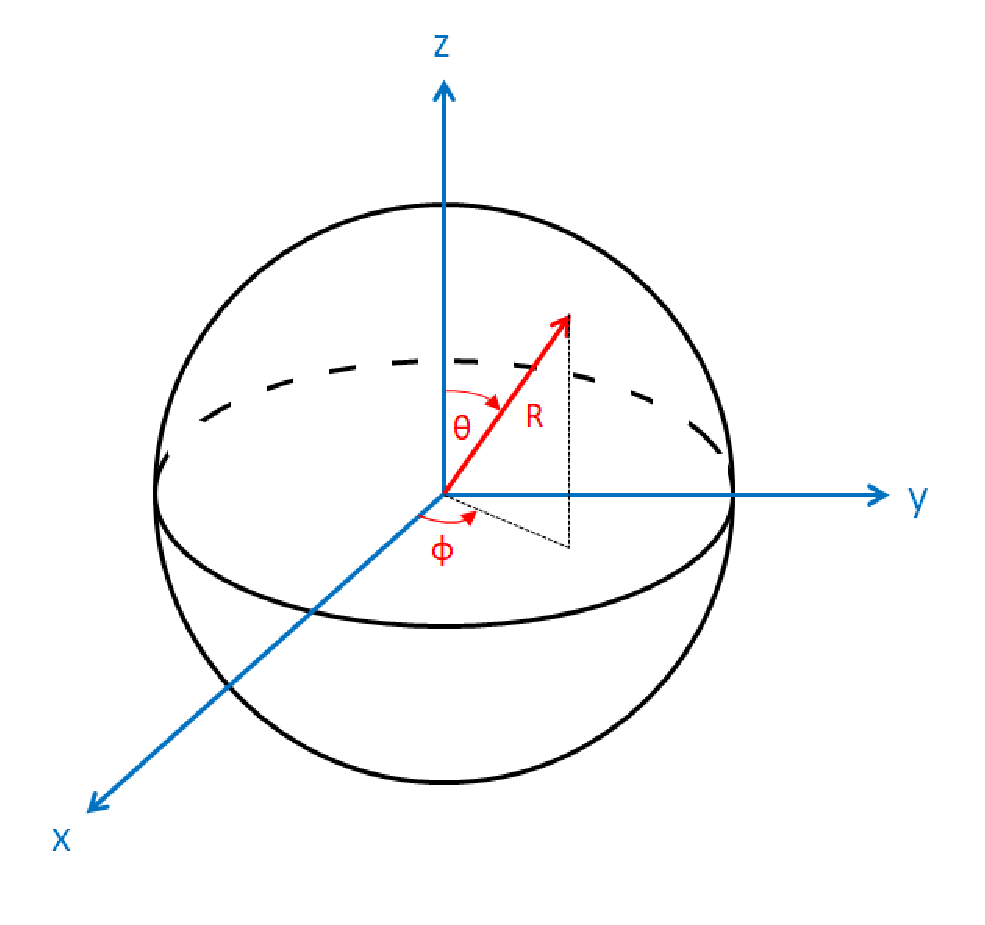
\includegraphics[width=7cm]{Figures/polar_coordinates.eps}
      \caption{Polar Coordinates}
      \label{polar_coordinates}
   \end{center}
\end{figure}

The magnetic field can be then expressed as follows:

\begin{equation}
\begin{aligned}
\hat{B}	&= -\mu_0\hat{\nabla} V(\hat{r})\\
		&= -\mu_0 \cdot \Big( \frac{dV}{dr} , \frac{1}{r}\frac{dV}{d\theta} , \frac{1}{r\sin(\theta)}\frac{dV}{d\phi} \Big)\\
		&= \Big(- \frac{2\mu_0M\cos(\theta)}{4\pi r^3} , - \frac{\mu_0M\sin(\theta)}{4\pi r^3} , 0\Big)
\end{aligned}
\end{equation}
and the total field is:
\begin{equation}
B(r,\theta,\phi) = \frac{\mu_0M}{4\pi r^3} \sqrt{1 + 3\cos^2(\theta)}
\end{equation}

If the planet's radius is equal to $R_P$, the magnetic field at the planet's surface can be expressed as follows:

\[
\left\{
\begin{array}{r c l}
B_r & = & 2B_0\cos(\theta)\\
B_{\theta} & = & B_0\sin(\theta)\\
B_{\phi} & = & 0
\end{array}
\right.
\]
where 
\begin{equation}
B_0 = -\frac{\mu_0M}{4\pi R_P^3}
\end{equation}

The value of $B_0$ is directly proportional to $M$ and inversely proportional to the radius of the planet. For Earth, $M=1$ and $B_0 = -30.5 \mu T = -0.305\,Gauss$. On the other hand, currently, on Mars, $M_0 \approx -0.0002$ and $B_0 \approx -30 NT$ \cite{van1999planetary}

As we will discuss later on, the solar wind exerts a magnetic and dynamic pressure ($P_B$ and $P_D$) on objects in the space, including planets. These expressions are given by:

\[
\left\{
\begin{array}{r c l}
P_B & = & B^2 / 2\mu_0\\
P_D & = & 1/2 \rho v^2\\
\end{array}
\right.
\]

If we treat the solar's magnetic field as a dipole, we can express the field at a given point as as $ B = B_S / r^3$, where r is the distance from the sun to the given point. Thus, the magnetic pressure $P_B$ is inversely proportional to $r^6$ making it way smaller than $P_D$ which is inversely proportional to $r^2$ for large distances. $P_B$ can therefore be neglected.

The dynamic pressure, on the other hand, has an effect on the planets and comets within the solar system. This effect depends on the nature of the object (whether or not it has an atmosphere and/or a magnetic field). Fig. \ref{planets_types} shows the different possibilities that can exist: an object might have no magnetic field nor an atmosphere (a); it might have a very thing atmosphere but no magnetic field; or it might have an atmosphere and a magnetic field.

\begin{figure}
   \begin{center}
      \includegraphics[width=9.5cm]{Figures/planets.png}
      \caption{Different Possibilities for a planet: (a) A Planet with no Magnetic Field nor an Atmosphere; (b) A Planet with an Atmosphere but no Magnetic Field; (c) A Planet with an Atmosphere and a Strong Magnetic Field}
      \label{planets_types}
   \end{center}
\end{figure}

With the first case out of question, focus is placed mainly on the second and third case.

\paragraph{No Magnetic Field, but Atmosphere Present}\label{nomagatm}

Mars currently has no magnetic field but a thin atmosphere. The atmosphere of Mars currently consists of a very thin layer of gas that exerts a pressure at the surface equal to $0.006atm$. The equilibrium state between the atmospheric pressure and solar wind pressure suggests that these two are equal:
\begin{equation}
P_{ap} = P_{sw}
\end{equation}
where $P_{ap}$ is the atmospheric pressure and $P_{sw}$ is the pressure due to the solar wind. These pressures act mainly in the ionopause. The solar Extreme UltraViolet (EUV) radiations hit the upper layers of the atmosphere. EUV are radiations whose wavelengths are between 10nm and 120nm and are highly energetic. Upon hitting the upper layers of the atmosphere, not only do they heat it, but they also ionize it, creating the ionosphere.

As we stated above, Mars has no magnetic field and a very thin atmosphere. Thus, it is interesting to study the current state of the atmosphere to derive how high the ionopause can be, and whether or not the solar wind is capable of hitting Mars's surface (very low ionopause).

If we assume a hydrostatic equilibrium in the planetary atmosphere:
\begin{equation}
\frac{dP}{dr} = -\rho g
\end{equation}
where $\rho = nm$ is the (mass) density of air ($n$ is the density in number of particles per unit of volume and $m$ is the mass of one particle) and the pressure $P = nkT$, which gives us $\rho/m = P/kT$, thus:

\begin{equation}
\frac{dP}{dr} = \frac{Pmg}{kT}
\end{equation}
or again
\begin{equation}
\frac{dP}{P} = \frac{mg}{kT} dr
\end{equation}

If we integrate both sides, we get:
\begin{equation}
\int_{P_0}^P \frac{dP}{P} = -\frac{mg}{kT}\int_{r_0}^r dr
\end{equation}
 where $P_0$ is the pressure at the surface of the planet, and $r_0$ the radius of the planet.
 
which gives us again:
\begin{equation}
ln\Big(\frac{P}{P_0}\Big) = - \frac{mg}{kT}(r - r_0).
\end{equation}
Therefore, we could derive the expression of the pressure at any point from the planet's center:

\begin{equation}
P(r) = P_0 ^{-\frac{mg}{kT}(r-r_0)}.
\end{equation}
Calling $H=\frac{kT}{mg}$, this could translate into a function of the height $h$ where $h = r-r_0$ is the height from the planet's sufrace:

\begin{equation}
P(h) = P_0 ^{-\frac{h}{H}}.
\end{equation}

To recall, the ionopause is where the atmosphere has a gas pressure that balances the solar pressure. In other words, at this height, $P_{ap} = P_{sw}$. As stated above, the pressure due to the solar wind is $P_{sw} = \frac{1}{2} \rho_{sw}v_{sw}^2 = \frac{1}{2}n_{sw}m_{sw}v{sw}^2$. This gives us:

\begin{equation}
\label{equality}
P_0 ^{-\frac{h}{H}} = \frac{1}{2} n_{sw}m_{sw}v_{sw}^2.
\end{equation}

From eq. (\ref{equality}) we could derive the equation of the height of the ionopause:

\begin{equation}
h_{pa} = H \cdot ln\Big(\frac{2P_0}{n_{sw}m_{sw}v_{sw}^2}\Big)
\end{equation}

Given the following values:
\[
\left\{
\begin{array}{r c l}
n_{sw} & = & 10^6 m^{-3} \\
m_{sw} & = & 1.6726 \times 10^{-27} Kg \\
v_{sw} & = & 100\sim350 km\,s^{-1} \\
T & = & 200K \\
n_{ap} & = & 3 \times 10^{10} m^{-3} \\
m_{ap} & \approx & 7.3065 \times 10^{-26} Kg
\end{array}
\right.
\]
we could tell that the ionopause on Mars is at a very low altitude. This means that solar wind radiations partially hit the surface of the planet, intoxicating it and making it uninhabitable. Thus, combined with the low gravity on Mars, the solar wind is capable of removing most of Mars' atmospheric molecules, even the heavy ones, leading to a low pressure and a very thin atmosphere.

\paragraph{Both a Field and an Atmosphere present}

Earth, however, has both a magnetic field and sufficiently thick atmosphere. Our home planet is perfect life to exist and develop: the gravity of the planet is strong enough and the planet has a magnetic field, contributing both to the creation and the maintenance of thick atmosphere. The surface pressure is also high enough for liquid water to exist under normal circumstances.

However, in general, the magnetic field can have a strength that depends on the state of the core of the planet. Assuming that we manage to create such a field on Mars, we try to estimate the optimal (or minimal) magnetic field strength required to maintain a certain atmospheric pressure at the surface, which would theoretically allow for life to sustainably exist. 

As mentioned above, we can approximate the magnetic field of a planet to a dipole. Subject to the solar wind, Mars' magnetic field would be modified, creating the protective magnetosphere. The outer boundary of the magnetosphere is what was referred to, above, as the magnetopause. However, unlike the previous case where the the solar wind interacts directly with the atmosphere, the side of the planet facing the sun (and facing the coming solar wind) has another boundary that is formed. This boundary is due to the fact that the solar wind is supersonic and is called the \textit{``bow shock''}. This is shown in Fig. \ref{planets_types} (c).

In this case, the magnetic field pressure is the one that balances the pressure due to the solar wind, i.e.
\begin{equation}
P_m = P_{sw}
\end{equation}
where $P_m = B^2 / 2 \mu_0$.

To recall, B was found previously in eq. (5) to vary as $\frac{B_0}{r^3}$. This gives us the expression of the magnetic field pressure, on the equator, to be:
\begin{equation}
P_m = \frac{B_0^2}{2\mu_0\cdot r^6}
\end{equation}

Also, we have previously mentioned that the solar pressure is $P_{sw} = \frac{1}{2}\rho_{sw}v_{sw}$ where $\rho_{sw} = n_{sw}m_{sw}$. This gives us:
\begin{equation}
\frac{B_0^2}{2\mu_0\cdot r^6} = \frac{1}{2}n_{sw}m_{sw}v_{sw}
\end{equation}

From that, we can derive that the height of the magnetopause as a function of the radius of the planet:

\begin{equation}
r = \sqrt[6]{\frac{B_0^2}{\mu_0n_{sw}m_{sw}v_{sw}^2}}
\end{equation}
and:
\[
\begin{array}{r c l}
 & = & \sqrt[6]{\frac{B_0^2}{\mu_0n_{sw}m_{sw}v_{sw}^2}} - r_0 \\
 & = & \sqrt[6]{\frac{M_0^2}{4\pi n_{sw}m_{sw}v_{sw}^2}} - r_0\\
\end{array}
\]
where $r_0$ is the radius of the planet.

The magnetopause must be high enough so that any loss or escape of atmosphere on Mars will be only due to the low gravity. In other words, the vast majority of the planet's atmosphere should be at heights significantly lower than that of the magnetopause.

For now, we assume that the ionopause satisfies such a property. Thus, we can use an isothermal-barotropic approximation to model the atmosphere. This approximation depends highly on the composition of the planet's atmosphere. For now we will use the planet's current composition (i.e., $95\% \sim 96\% \,CO_2$), using $CO_2$'s molecular and molar mass to measure the planet's atmospheric pressure after stabilization with the introduction of a magnetic field.

To begin with, the atmosphere is assumed to be an ideal gas, satisfying the following equation:
\begin{equation}
\rho = \frac{M\,P}{R\,T}
\label{rho_function}
\end{equation}
where $\rho$ is the mass density, $M$ is the average molecular weight (i.e., that of $CO_2$ in our case) $P$ is the pressure, $T$ the temperature and R is the idea gas constant.

Later on, when performing the simulations, the temperature of the planet is $\sim47^{o}C$ or again $320^{o}K$ on average. This temperature is used for the model. Note that the model suggests that the temperature is invariant for all the points inside the atmosphere regardless of the altitude, which is not realistic. Nonetheless, while the temperature in reality varies depending on the season on the planet, from $\sim32^oC$ to $\sim62^oC$, this fact does not contradict the model itself, and will be taken into account later. 

Now that the solar wind pressure is practically cancelled due to the magnetic field, the gas of the planet's atmosphere is held in place by the hydrostatic forces. For a given height, the downwards forces of weight of the gas at higher altitudes is equal to the upwards force exerted by pressure in the layer below. This relation can be expressed as follows:
\begin{equation}
PA - (P + dP) A - (\rho Adh)g_0 = 0
\end{equation}
which can be simplified as:
\begin{equation}
dP = \rho g_0 dh
\end{equation}
where $g_0$ is the gravitational acceleration at the planet's surface.

If we replace $\rho$ by its expression given in eq. \ref{rho_function}, we get:
\begin{equation}
dP = \frac{M\,P}{R\,T} g_0 dh
\end{equation}
which gives:
\begin{equation}
\int_{P_0}^P \frac{dP}{P} = \int_{h_0}^{h}\frac{M}{R\,T} g_0 dh
\end{equation}
Therefore, for a given height h,
\begin{equation}
ln(\frac{P}{P0}) = \frac{M}{R\,T} g_0 h
\end{equation}

For the given model, density and pressure are an exponential function of altitude. The scale height, defined as the increase in altitude for the pressure and the density to drop by a factor of $1/e$ of their initial values is:
\begin{equation}
H = \frac{R\,T}{M\,g_0}
\end{equation}
If we want to find the altitude $h_{total}$ below which 99.9\% of the atmosphere exists:
\begin{equation}
6.90\approx Ln(1000) = \frac{M}{R\,T} g_0 h_{total}
\end{equation}
and:
\begin{equation}
h_{total} = 6.90 \cdot \frac{R\,T}{M\,g_0} 
\end{equation}

%...............................................................%
\subsubsection{The Magnetic Field: How Strong Should It Be?}\label{howstrong}
%...............................................................%

Here, we start our experiments by attributing to Mars an atmosphere with a pressure equal to $0.6 atm$. This translates into a total mass equal to $2.24\times10^{18} Kg$. We assume that we managed to make Mars have a high enough pressure. We will try different magnetic field strengths, and study how long that atmosphere will last before it gets taken away or what would be left of it after a long time.

With that being set, the planet's temperature rises to reach an average equal to 47$^{\circ}$, with a maximum equal to 62$^{\circ}$ in the planet's summer, and 32$^{\circ}$ in its winter as shown in Fig. \ref{temperature}. Here, it is important to mention that summer and winter in Mars are common all over the planet. Thus, the seasons are not mainly caused by the planet's tilt as in the case of Earth, but to the planet's actual distance from the Sun, which varies noticeably between 205 million Km and 249 million Km as shown in Fig. \ref{marsvssun}.

\begin{figure}
   \begin{center}
      \includegraphics[width=8.5cm]{Figures/temperature.eps}
      \caption{Temperature at the surface of Mars after setting the atmospheric pressure to 0.6 atm}
      \label{temperature}
   \end{center}
\end{figure}

\begin{figure}
   \begin{center}
      \includegraphics[width=8.5cm]{Figures/mars_distance.eps}
      \caption{Mars's Summer and Winter: Distance to the Sun}
      \label{marsvssun}
   \end{center}
\end{figure}

The high temperatures seen at the surface can be attributed to pre-setting the mass/pressure of the atmosphere to a certain value while maintaining its composition. In other words, the an atmosphere mainly consists of carbon dioxide: a greenhouse effect gas.

However, reducing temperatures is currently not the main target. Instead, the main goal is the identification of how strong the magnetic field needs to be to protect the planet's surface from the solar wind.

We start with a strong assumption that suggests that the relation between the magnetopause height on the dayside of the planet (i.e., $h_{pa}$) and the height below which 99.9\% of the atmosphere exists (i.e., $h_{total}$) is perfect on Earth. In other words, the ratio between these two needs to be satisfied on Mars for the magnetic field to be able to protect the planet from the solar wind.

From the previous sections we have established:

\[
\left\{
\begin{array}{r c l}
h_{pa}  & = & \sqrt[6]{\frac{M_0^2}{4\pi n_{sw}m_{sw}v_{sw}^2}} \\
h_{total} & = & 6.90 \cdot \frac{R\,T}{M\,g_0} 
\end{array}
\right.
\]

On Earth, $h_{pa} = 10 R_E$ where $R_E$ is the radius of Earth. It is roughly equal to $63,710Km$. The height below which 99.9\% of the atmosphere exists $h_{total}$ is about 50Km. The Radio between both is $\xi_{Earth} = \frac{10 radii}{50} \approx 1274$. For Mars, this translates into:
\begin{equation}
\xi_{Mars} = \frac{h_{pa}}{h_{total}} \approx 1274
\end{equation}

Given the following values:
\[
\left\{
\begin{array}{r c l}
R & = & 8.3144598 J\cdot mol^{-1}\cdot K^{-1} \\
T & = & 320.15 K \\
M_{CO_2} & = & 44.01\cdot 10^{-3} Kg\,mol^{-1} \\
g_0 & = & 3.73 N\cdot Kg^{-1}
\end{array}
\right.
\]

We can approximate the height below which 99.9\% of the atmosphere exists $h_{total} \approx 16.22 Km$. With reference to the ratio we established $h_{pa} \approx 1274 \times h_{total}$, we can derive the following equation to find the magnetic field strength required:
\begin{equation}
\begin{aligned}
\hat{B}	&= -\mu_0\hat{\nabla} V(\hat{r})\\
		&= -\mu_0 \cdot \Big( \frac{dV}{dr} , \frac{1}{r}\frac{dV}{d\theta} , \frac{1}{r\sin(\theta)}\frac{dV}{d\phi} \Big)\\
		&= \Big(- \frac{2\mu_0M\cos(\theta)}{4\pi r^3} , - \frac{\mu_0M\sin(\theta)}{4\pi r^3} , 0\Big)
\end{aligned}
\end{equation}

As we could observe in our experiment, the surface pressure, no matter how strong the magnetic field is, decreases over time. The highest obtainable stable pressure is equal to 0.38 atm, which is understandable given that Mars's gravity is 0.38 of that of earth.

However, this pressure would be problematic for the human body, and might suggest that a mask and a special suit may be required for human life (for reasons mentioned in \ref{sec:why} . However, fortunately, such a pressure is enough to liquify the frozen water on the surface, restoring part of Mars's old ocean and seas.

%...............................................................%
\subsubsection{The Magnetic Field: How?}
%...............................................................%

\paragraph{Melting Mars's core}
Mars does not have a magnetic field. While the common belief is that the frozen core of Mars is the main reason Mars lost its magnetic field. It has been believed that the conducting fluid in motion in the core of Earth is what generates its magnetic field: the melted core is rich of conducting metals (such us Fe and Ni), whose electrons are released by friction and heat. These electrons in massive motion make the Earth's magnetic field.

However, at the same time this notion has been subject to different objections for iron loses its magnetic properties when heated \cite{velasco2007}. In fact, liquid iron is very different from solid iron, and it can not be, under any condition, magnetic.
 
Nevertheless, having properties similar to that of Earth, including a melted core, could reproduce the magnetic field of Earth. There are three main properties for a planet to have a magnetic field:

\begin{itemize}
\item A liquid core
\item A core rich in metals
\item A high enough rotation rate
\end{itemize}

Elon Musk, as well as many others, has proposed to bomb the core of Mars with nuclear bombs \cite{griffin2015}. Some studies have shown that such procedure requires almost $10^{29} J$ or approximately $10^{13} Megatons$, which is practically impossible. To recall, Tsar Bomba, the biggest nuke built, could produce only a damage equal to $50 Megatons$ \cite{biello2007need}. 

\paragraph{Surrounding Mars with a Metallic Wire Carrying Electric Current}
A circular wire carrying electricity creates a magnetic field that is very similar to that required for Mars' terraforming. Having a long wire going around Mars as shown in Fig. \ref{wire} could possibly generate a magnetic field if an electric current runs through it.

\begin{figure}
   \begin{center}
      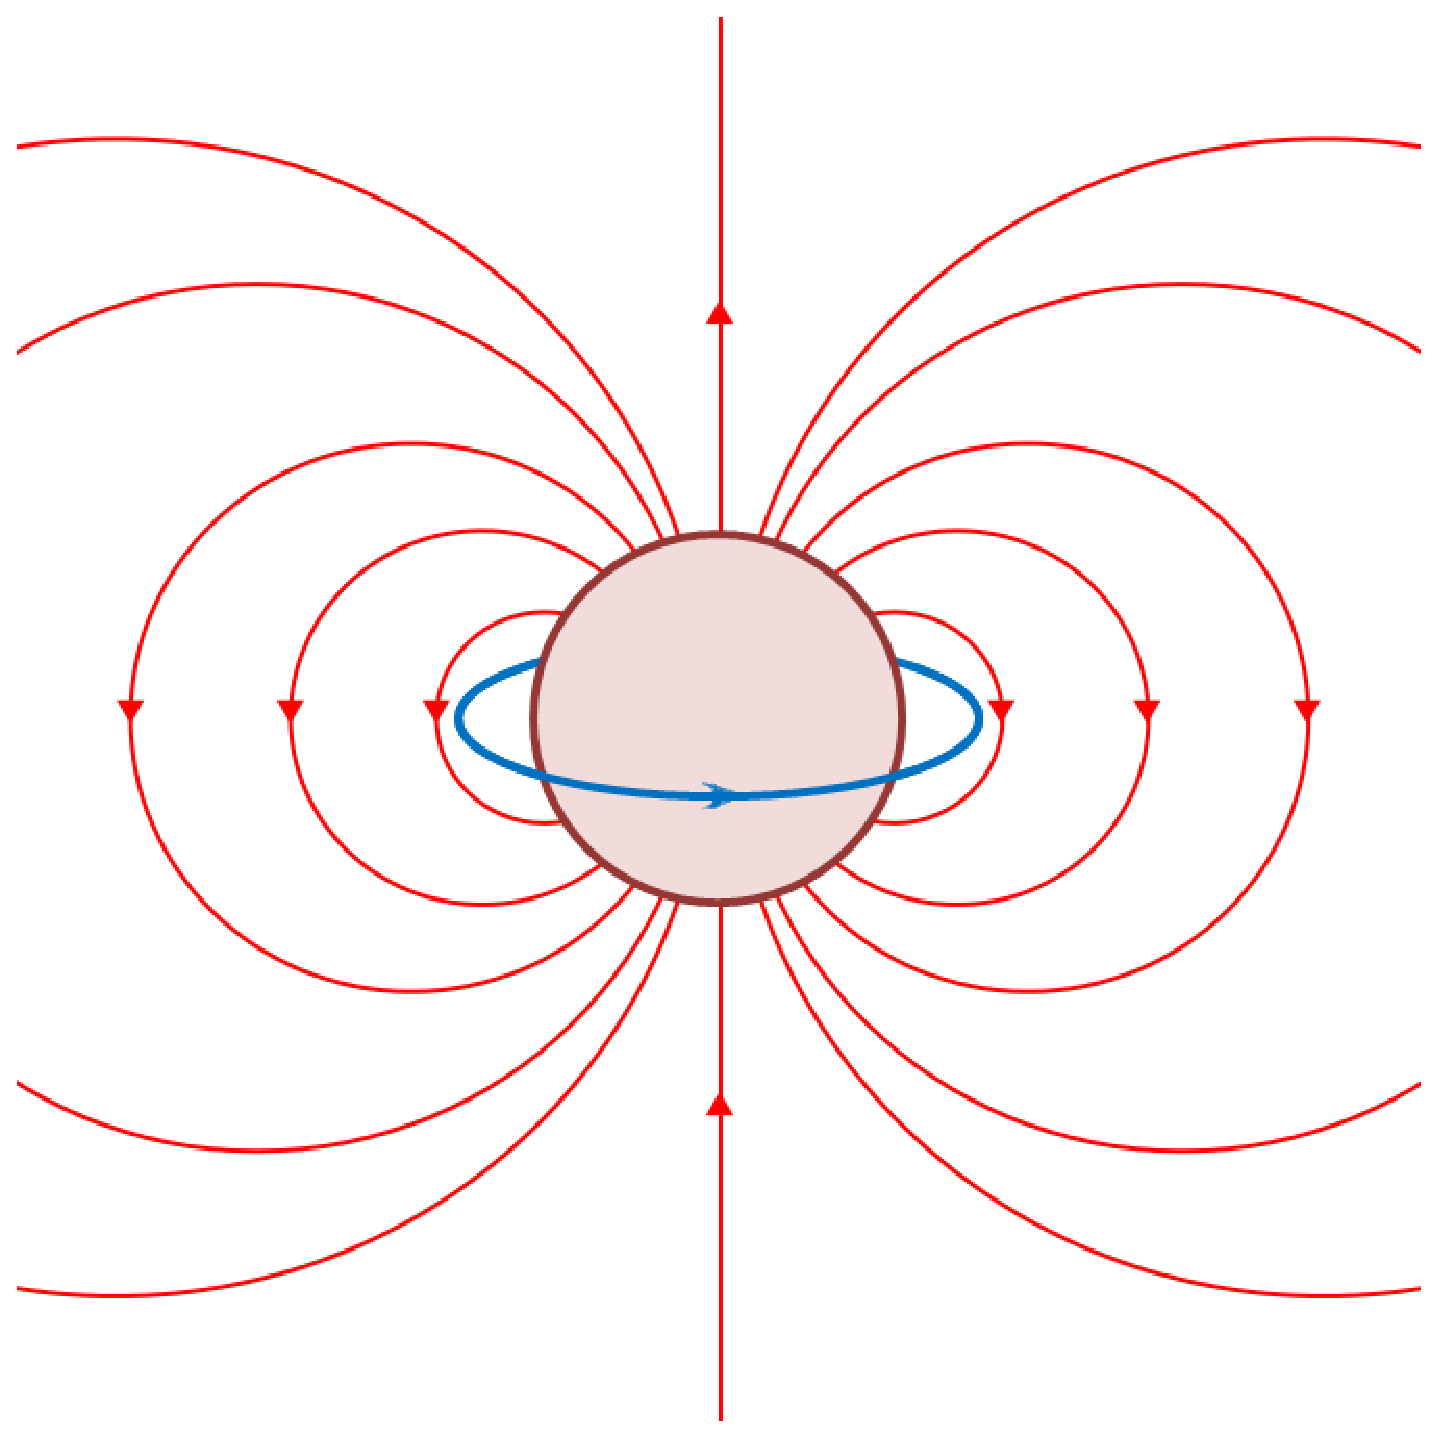
\includegraphics[width=7.5cm]{Figures/magnetic_ring.eps}
      \caption{Proposed Approach to Use Induction to Create a Magnetic Field on Mars}
      \label{wire}
   \end{center}
\end{figure}

However, as with the previous approach, this approach is demanding: such a long wire should be thick enough to make sure that its resistance will not consume the total amount of electricity. Nevertheless, the electric current required to circulate through a wire that goes over all the planet (21\,343 Km at least) is technically impossible to produce on the planet without having installed the required equipment prior to the terraforming procedure. 

\paragraph{Using A Magnet Satellite}
This proposal is a bit more challenging, yet more feasible than the previous ones, and do not require similar huge amount of energy

%====================================================%
\section{Experimental Results}\label{sec:results}
%====================================================%

%--------------------------------------------------------------%
\subsection{Current State of Mars}\label{currentstate}
%--------------------------------------------------------------%
In section \ref{nomagatm}, we have found the height of the ionopause in absence of a magnetic field to be:
\begin{equation}
h_{pa} = H \cdot ln\Big(\frac{2P_0}{n_{sw}m_{sw}v_{sw}^2}\Big)
\end{equation}

The ionopause height was found to be ___ given the following values:
\[
\left\{
\begin{array}{r c l}
n_{sw} & = & 10^6 m^{-3} \\
m_{sw} & = & 1.6726 \times 10^{-27} Kg \\
v_{sw} & = & 100\sim350 km\,s^{-1} \\
T & = & 200K \\
n_{ap} & = & 3 \times 10^{10} m^{-3} \\
m_{ap} & \approx & 7.3065 \times 10^{-26} Kg
\end{array}
\right.
\]

This height is very low to a point where the solar wind radiations will partially hit the surface, intoxicating it and worsening the potential environment for human life. 

In Fig. \ref{mars_before}, we show the current physical state of Mars with no magnetic field as simulated by \textit{Universe Sandbox}$^2$. The atmospheric pressure reported is 0.00673 atm, and the mass loss rate is equal to $30Kg\cdot s^{-1}$.

\begin{figure}
   \begin{center}
      \includegraphics[width=8.5cm]{Figures/oldmars.png}
      \caption{Current State of Mars}
      \label{mars_before}
   \end{center}
\end{figure}

%--------------------------------------------------------------%
\subsection{Mars After the Establishment of an Atmosphere (No Magnetic Field)}
%--------------------------------------------------------------%
In this subsection, we suppose that a sufficiently thick atmosphere has been established, with the surface pressure equal to 0.6 atm. Changes were observed: the temperature rose to reach an average of $47^{o}C$, with temperatures reaching $62^{o}C$ in the summer and $32^{o}C$ in the winter. However, with the increasing mass loss rate, the planet quickly started to lose its atmosphere, leading to a decrease in temperature. This decrease ultimately resulted in a reversion to an environment similar to that described in subsection \ref{currentstate} within a few decades. 

%--------------------------------------------------------------%
\subsection{Mars After the Establishment of an Atmosphere and a Magnetic Field}
%--------------------------------------------------------------%
We have previously established, in section \ref{howstrong}, the following two equations that determine the height of the magnetopause and the height under which 99.9\% of the atmosphere exists: 
\[
\left\{
\begin{array}{r c l}
h_{pa}  & = & \sqrt[6]{\frac{M_0^2}{4\pi n_{sw}m_{sw}v_{sw}^2}} \\
h_{total} & = & 6.90 \cdot \frac{R\,T}{M\,g_0} 
\end{array}
\right.
\]

We also supposed that the relation between the two is:
\begin{equation}
 h_{pa}= 1274 \cdot h_{total}
\end{equation}

Therefore, we can relate the height of the magnetopause to the temperature, giving the following equation:
\begin{equation}\label{heighteqn}
M_0= \sqrt{\big(\frac{8790.6\cdot R\,T}{Mg_0}\big)^6 \times 4\pi n_{sw}m_{sw}v_{sw}^2}
\end{equation}

As we stated above, the temperature after the establishment of the atmosphere varies between $\sim32^oC$ and $\sim62^oC$. These are the maximum and minimum temperatures used in the simulations to find the height of the magnetopause. In Fig. \ref{magnetoheight}, we show the optimal height for the magnetopause considering these two limits. Understandably, we used the upper limit to make sure that the magnetopause is always high enough to protect the planet from solar winds.

The values below were then substituted into equation \ref{heighteqn}:
\[
\left\{
\begin{array}{r c l}
n_{sw} & = & 10^6 m^{-3} \\
m_{sw} & = & 1.6726 \times 10^{-27} Kg \\
v_{sw} & = & 100\sim350 km\,s^{-1} \\
T & = & 200K \\
n_{ap} & = & 3 \times 10^{10} m^{-3} \\
m_{ap} & \approx & 7.3065 \times 10^{-26} Kg
\end{array}
\right.
\]

The optimal $M_0$, the magnetic moment, found was equal to .... This magnetic moment corresponds to a magnetic field of strength equal to ... Gauss.
 
Using this value for the magnetic field and a value for the atmospheric pressure equal to 0.6 atm for  \textit{Universe Sandbox}$^2$ simulations, the mass loss was minimal. The minimal mass loss translates to an atmosphere of stable thickness, as seen in Fig. \ref{newmars}. However, it must be noted that in the figure, water was added to the planet (part of it is included in the atmosphere in form of water vapors).

\begin{figure}
   \begin{center}
      \includegraphics[width=8.5cm]{Figures/newmars.png}
      \caption{State of Mars After the Establishment of Atmosphere and Magnetic Field}
      \label{newmars}
   \end{center}
\end{figure}


%====================================================%
\section{Conclusion}\label{sec:conclusion}
%====================================================%
Scientists, researchers, and the public have started discussions on the possible colonization of other planets, mainly Mars, in the future. However, several evident obstacles impede the hope for human life, including the lack of a substantial atmosphere and magnetic field, necessary temperatures, and liquid water. This study mainly dealt with uncovering the necessary strength of magnetic fields and heights of the atmosphere required to ensure that Mars' atmosphere is stable and thick enough to sustain human life. Ultimately, the height at which 99.9\% of the atmosphere must exist was found to be ___, while the magnetic field strength was found to be ____. In addition, the temperature fluctuations experienced on the planet could be found using \textit{Universe Sandbox}$^2$ and \textit{Matlab}.

However, it is important to notice that this study only covers the importance of a magnetic field, not how to create the atmosphere in the first place. Several approaches on how to have liquid water on the planet have been proposed in literature. In fact, there has been indication of large masses of water ice under lobate debris aprons on the planet \cite{evidenceice}. Perhaps, future studies can help indicate whether the establishment of the atmosphere and pressure as proposed in this paper will provide the sufficient conditions to melt the ice. Other proposals include the construction of 'orbital mirrors', which would reflect sunlight on the the planet?s surface, ultimately increasing the surface temperature \cite{zubrin1997technological}. At the same time, theoretical physicist Dr. Michio Kaku has even proposed carefully shooting asteroids and comets at Mars to release water while trying to minimize surface damage\cite{kaku2010}.

% =============================
% ***             BIBLIOGRAPHY             ***
% =============================

\bibliography{reference}

\end{document}


